\documentclass[11pt]{article}
\usepackage[a4paper,margin=2cm]{geometry}
\usepackage{amsmath,amssymb,booktabs,array,float}
\usepackage{tikz}
\newcommand{\Cg}{\mathcal{C}_{\mathrm{GME}}}
\newcommand{\rdm}{\Gamma^{(n)}}
\setlength{\parindent}{0pt}
\setlength{\parskip}{5pt}
\begin{document}
\sloppy

\section*{Building $\rdm$ from its symmetries instead of all $4^n$ elements}

For a cluster of $n$ sites the $n$-spin RDM is built element by element from the state $|\Psi\rangle$,
\begin{equation}
  \rdm_{\sigma',\sigma}=\Big\langle\Psi\Big|\prod_{k=1}^{n}d^{\dagger}_{k,\sigma'_k}\,d^{\phantom\dagger}_{k,\sigma_k}\Big|\Psi\Big\rangle
  \equiv\langle\Psi|\hat O_{\sigma',\sigma}|\Psi\rangle ,
  \qquad \rho_s=\frac{\rdm}{\mathrm{Tr}\,\rdm},
  \label{eq:gamma}
\end{equation}
where $\sigma=(\sigma_1,\dots,\sigma_n)$ and $\sigma'$ run over the $2^n$ spin configurations of the
cluster. Computing every element costs $4^n$ expectation values per cluster. Three exact properties of
$\rdm$ reduce this number; none of them changes $\rho_s$.

\textbf{1.\ $S_z$ blocks.} Let $d(\sigma)$ be the number of down spins in $\sigma$ and $m(\sigma)=\tfrac12\big(n-2d(\sigma)\big)$
its $S_z$. The pair $d^\dagger_{k,\sigma'_k}d_{k,\sigma_k}$ removes a spin $\sigma_k$ and adds a spin
$\sigma'_k$ on site $k$, so the product in Eq.~(\ref{eq:gamma}) changes the total $S_z$ by
\begin{equation}
  [\hat S_z,\hat O_{\sigma',\sigma}]=\big(m(\sigma')-m(\sigma)\big)\,\hat O_{\sigma',\sigma}.
\end{equation}
Applied to a state with definite $\hat S_z$ it gives a state with a different $\hat S_z$ unless
$m(\sigma')=m(\sigma)$, and the overlap with $|\Psi\rangle$ vanishes:
\begin{equation}
  \rdm_{\sigma',\sigma}=0\qquad\text{if } d(\sigma')\neq d(\sigma).
  \label{eq:sz}
\end{equation}
Ordered by $d$, $\rdm=\bigoplus_{d=0}^{n}\rdm_{[d]}$ is block diagonal, with blocks of size
$\binom{n}{d}$. A thermal state $\rdm(T)=\sum_m p_m(T)\,\rdm[\psi_m]$ commutes with $\hat S_z$ as
well. Elements to compute: $\sum_d\binom{n}{d}^2=\binom{2n}{n}\approx 4^n/\sqrt{\pi n}$.

\textbf{2.\ Hermiticity.} $\hat O_{\sigma',\sigma}^\dagger=\hat O_{\sigma,\sigma'}$, hence $\rdm_{\sigma,\sigma'}=\big(\rdm_{\sigma',\sigma}\big)^{*}$. The
Hubbard Hamiltonian is real, so $|\Psi\rangle$ and $\rdm$ are real and $\rdm_{\sigma,\sigma'}=\rdm_{\sigma',\sigma}$.
Only the diagonal and the upper triangle of each block are computed; the lower triangle is a copy.

\textbf{3.\ Spin flip.} Let $\hat F$ exchange the up and down orbital on every site, $\hat F d^\dagger_{k,\sigma}\hat F^\dagger=d^\dagger_{k,\bar\sigma}$,
and let $\bar\sigma$ be $\sigma$ with every spin flipped. Then
$\hat F\hat O_{\sigma',\sigma}\hat F^\dagger=\hat O_{\bar\sigma',\bar\sigma}$. The Hamiltonian treats $\uparrow$ and
$\downarrow$ alike, $[\hat H,\hat F]=0$, and $\hat F$ maps the $S_z=0$ sector onto itself, so a
non-degenerate $S_z=0$ eigenstate satisfies $\hat F|\Psi\rangle=\pm|\Psi\rangle$. Therefore
\begin{equation}
  \rdm_{\bar\sigma',\bar\sigma}=\langle\Psi|\hat F\hat O_{\sigma',\sigma}\hat F^\dagger|\Psi\rangle
  =(\pm1)^2\,\rdm_{\sigma',\sigma}=\rdm_{\sigma',\sigma}.
  \label{eq:flip}
\end{equation}
The sign of $\hat F|\Psi\rangle$ cancels, so the relation holds for singlets and for $S_z=0$ triplet
components alike. It maps block $d$ onto block $n-d$: only the blocks with $d\le n/2$ are computed,
and the middle block ($d=n/2$, even $n$) only up to the flip. Eq.~(\ref{eq:flip}) also holds for a
ground state averaged over its degenerate manifold and for thermal states, since $[\hat H,\hat F]=0$.

For $n=2$ the configurations, ordered by $d$, are $\uparrow\uparrow$; $\uparrow\downarrow,\downarrow\uparrow$; $\downarrow\downarrow$.
Of the $16$ elements, $10$ vanish by Eq.~(\ref{eq:sz}) and the remaining $6$ carry only three numbers:

\begin{center}
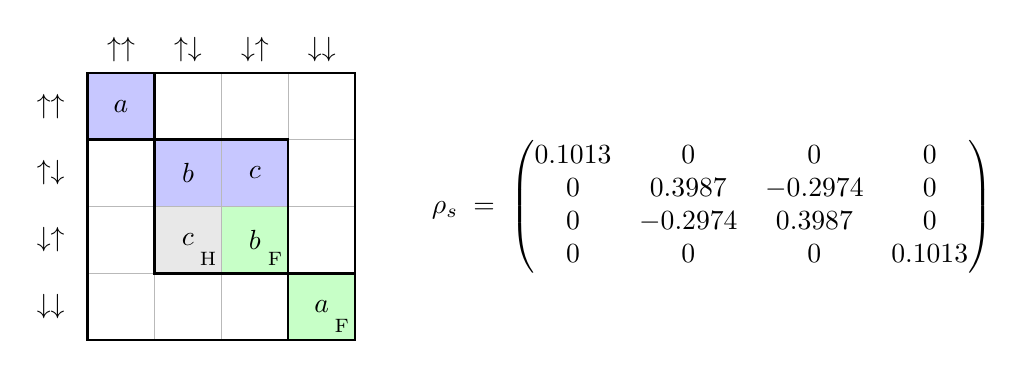
\begin{tikzpicture}[x=0.85cm,y=0.85cm]
  \foreach \i/\lab in {0/{\uparrow\uparrow},1/{\uparrow\downarrow},2/{\downarrow\uparrow},3/{\downarrow\downarrow}}{
    \node at (\i+0.5,4.35) {$\lab$};
    \node at (-0.55,3.5-\i) {$\lab$};
  }
  \fill[blue!22]  (0,3) rectangle (1,4);
  \fill[blue!22]  (1,2) rectangle (3,3);
  \fill[green!22] (2,1) rectangle (3,2);
  \fill[green!22] (3,0) rectangle (4,1);
  \fill[gray!18]  (1,1) rectangle (2,2);
  \draw[step=1,gray!55] (0,0) grid (4,4);
  \draw[thick] (0,0) rectangle (4,4);
  \draw[thick] (0,3) rectangle (1,4); \draw[thick] (1,1) rectangle (3,3); \draw[thick] (3,0) rectangle (4,1);
  \node at (0.5,3.5) {$a$}; \node at (1.5,2.5) {$b$}; \node at (2.5,2.5) {$c$};
  \node at (1.5,1.5) {$c$}; \node at (2.5,1.5) {$b$}; \node at (3.5,0.5) {$a$};
  \node[font=\scriptsize] at (1.8,1.22) {H}; \node[font=\scriptsize] at (2.8,1.22) {F}; \node[font=\scriptsize] at (3.8,0.22) {F};
  \node[anchor=west] at (5.0,2) {$\displaystyle
   \rho_s\;=\;\begin{pmatrix}
     0.1013 & 0 & 0 & 0\\
     0 & 0.3987 & -0.2974 & 0\\
     0 & -0.2974 & 0.3987 & 0\\
     0 & 0 & 0 & 0.1013
   \end{pmatrix}$};
\end{tikzpicture}
\end{center}

{\small Blue: computed ($a$, $b$, $c$). Grey, H: copy by hermiticity, a mirror across the diagonal;
it never relates two diagonal elements. Green, F: copy by the spin flip, Eq.~(\ref{eq:flip}), which maps
$\uparrow\uparrow\to\downarrow\downarrow$ and $\uparrow\downarrow\to\downarrow\uparrow$ and therefore also relates diagonal elements,
$\rdm_{\downarrow\downarrow,\downarrow\downarrow}=\rdm_{\uparrow\uparrow,\uparrow\uparrow}$ and
$\rdm_{\downarrow\uparrow,\downarrow\uparrow}=\rdm_{\uparrow\downarrow,\uparrow\downarrow}$. Right: the stored $\rho_s$ for
$L=6$, $U/t=10$, ground state, in the same order; the equal entries are exactly the pairs above.}

Together the three properties leave about one twentieth of the elements:

\begin{table}[H]
\centering
\begin{tabular}{c r r r r r c}
\toprule
$n$ & all, $4^n$ & $S_z$ blocks & $+$ hermiticity & $+$ spin flip & saving & $L=10$, one cluster$^{\dagger}$ \\
\midrule
5 & 1\,024   & 252     & 142     & 71      & $14\times$ & 2.9 min $\to$ 12 s \\
6 & 4\,096   & 924     & 494     & 252     & $16\times$ & 12 min $\to$ 43 s \\
7 & 16\,384  & 3\,432  & 1\,780  & 890     & $18\times$ & 46 min $\to$ 2.5 min \\
8 & 65\,536  & 12\,870 & 6\,563  & 3\,299  & $20\times$ & 3.1 h $\to$ 9 min \\
9 & 262\,144 & 48\,620 & 24\,566 & 12\,283 & $21\times$ & 12 h $\to$ 35 min \\
\bottomrule
\end{tabular}

\smallskip
{\small $^{\dagger}$ cost of the present element-by-element construction at $L=10$, $U/t=10$
(sector dimension $63\,504$): $0.17$ s per element.}
\end{table}

For $n=L$ no expectation values are needed: $\rho_s$ is the pure state $\hat P|\Psi\rangle$, with
$\hat P$ the projector on singly occupied sites. On the ring a single cluster suffices, because the
cluster average equals one cluster for a translation-invariant state ($10^{-17}$ at $L=6$).

In practice: group the configurations by $d(\sigma)$; compute $\rdm_{\sigma',\sigma}$ with
$\sigma'\le\sigma$ in the blocks $d<n/2$, and in the block $d=n/2$ one pair of each
$\{(\sigma',\sigma),(\bar\sigma',\bar\sigma)\}$; fill the lower triangles by hermiticity and the blocks
$d>n/2$ by Eq.~(\ref{eq:flip}); set all elements between different blocks to zero; normalise and pass the
full $2^n\times2^n$ matrix $\rho_s$ to the GCG.

The three properties were checked on the stored RDM bank ($L=6$, $S_z=0$ sector, $U/t=4$ and $10$,
ground state and first excited state, $n=2,\dots,5$). Every element with $d(\sigma')\neq d(\sigma)$ is
exactly $0$ (also for $n=6$); $\max|\rdm-(\rdm)^{\mathsf T}|\le4\times10^{-17}$ and $\mathrm{Im}\,\rdm=0$;
$\max|\rdm_{\bar\sigma',\bar\sigma}-\rdm_{\sigma',\sigma}|\le8\times10^{-15}$, while
$\max|\rdm_{\bar\sigma',\bar\sigma}+\rdm_{\sigma',\sigma}|\ge0.24$, so the sign in Eq.~(\ref{eq:flip}) is $+$.

The convex roof $\Cg(\rho_s)$ cannot be split into blocks: the optimal decomposition
$\rho_s=\sum_i p_i|\Phi_i\rangle\langle\Phi_i|$ may mix different $S_z$. The symmetries only reduce the
construction of $\rdm$ (and the eigendecomposition of $\rho_s$); the GCG still receives the full
$2^n\times2^n$ matrix.

\end{document}
